\chapter{引言}

\section{研究背景与意义}
随着互联网、移动设备等科技的发展,数据以爆炸性的速度在增长。这些日益增长的数据背后隐藏着许多重要的信息,各个领域,例如商业、科学、医疗等,对信息的统计分析挖掘有着很高的热情。联机分析处理(OLAP) \cite{chaudhuri1997overview} 是一种多维度的数据分析技术,能进行大规模数据的分析及统计计算,多用于决策支持系统和数据仓库。\cite{wu2012avatara} \cite{sumbaly2013big}

%例如企业可分别从用户维度,产品维度以及订单维度来分析对于不同年龄阶层最受欢迎的产品类型,从而推出针对不同年龄阶层的产品销售计划。由于企业数据的快速增长和累积以及企业对分析历史数据、挖掘商业价值的热情逐渐增高,联机分析处理应用在业界变得越来越受欢迎,开发更高效的 OLAP 技术浪潮应运而生。

数据立方(Data Cube) \cite{gray1997data} 是由 Jim Gray 等人于 1996 年提出的,它是一种有效支持 OLAP 应用的多维数据计算模型,是 OLAP 领域中的一项关键技术。它提出通过预先计算数据表中各属性间的所有组合对应的 GroupBy 结果并将其存储起来,从而缩短系统的查询响应时间,提高应用效率。

GroupBy 操作是多维数据在统计分析时常用的操作,它通过对具有相同属性值的数据进行聚合计算,从而统计分析不同维度不同特征的数据。由于GroupBy操作针对的都是历史数据,这些数据一般而言是不会变动的。同时,大部分的GroupBy结果很可能会被反复查询,若每一次的查询都从原始数据表中扫描计算,会耗费非常多的时间并占用不必要的计算资源。如果将这些统计信息预先计算并且存储起来,则之后的每一次查询都可从已计算好的结果中直接读取获得,从而可缩短查询响应时间和节省计算资源。

例如对于一张关于销售记录的关系表,会有以下几个属性(Product, Store, Customer, Sales)  \cite{beyer1999bottom}。销售人员除了关心总体的销售量外,还可能想知道各个Product、Store、Customer的销售量,这些信息的统计需要进行 GroupBy(Product), GroupBy(Store), GroupBy(Customer) 的聚合计算,这里的聚合函数是SUM,需要进行求和计算的属性是Sales。除此以外,销售人员可能还想了解多个维度组合的聚合计算的结果,例如某个商品在某个店铺的销售量、某个用户在某个店铺的消费量等。这些多维度组合的聚合计算包括GroupBy(Product, Store), GroupBy(Product, Customer), GroupBy(Store, Customer) 和 GroupBy(Product, Store, Customer)。这些所有的 GroupBy 结果构成了数据立方。将这些计算好的 GroupBy 结果存储于数据库中,销售人员或者公司高层即可根据各自需要快速查询不同维度组合的销售信息。在 SQL 中可用 CUBE ON 语句表示以上的操作。

\begin{verbatim} 
SELECT Product, Store, Customer, SUM(Sales)
FROM 'sales.table'
CUBE ON Product, Store, Customer
\end{verbatim}

在OLAP术语中,聚合的属性称为维属性,被计算的属性称为度量属性。在上述销售表中,Product,Store,Customer均为维属性,Sales为度量属性。

随着统计分析复杂性的增加,仅使用代数度量函数已无法满足统计分析的需求。代数度量指可将数据轻易拆分成多个子块进行计算的度量,如SUM(a+b)=SUM(a)+SUM(b)。许多对日志等复杂数据进行分析的度量函数多为整体性度量函数,如DISTINCT, TOPK等。 以下是 \cite{nandi2011distributed}  中一个对搜索日志进行分析查询的例子。

\begin{verbatim} 
SELECT COUNT(DISTINCT(User)), COUNT(*)
FROM 'log.table'
CUBE ON Location, Query
HAVING COUNT(DISTINCT(User)) > 5
\end{verbatim}

该查询涉及到了搜索日志中(Location, Query, User)这三个属性,其中 Location 和 Query 为维属性,User为度量属性。该查询对 Location 与 Query 进行数据立方计算,计算各组聚合数据中不同的 User 的数量以及各组聚合数据的数量。这一类查询关注的是搜索频率不高但搜索用户覆盖较广的内容。部分的搜索内容由于搜索频率不高,在进行分析统计时往往很容易被忽略。但由于这些内容被大部分用户(即很多不同的用户)搜索过,因此应该在分析统计时给予关注。在这个例子中,使用的COUNT(DISTINCT(User))正是一个整体性度量函数,它需要综合整组数据进行统计计算,而无法像代数度量简单地对数据进行拆分计算。%在之后的小节中,将对这两种类型的度量给出明确的定义。

以上无论是销售量统计或者搜索频率统计,这些统计信息都是多个维度多种组合的 GroupBy 计算,并且这些 GroupBy 组合之间是有一定联系的。如果我们能够利用各个GroupBy组合之间的一些共享关系进行计算,就能达到提高计算效率的目的,而这正是数据立方的核心思想所在。

随着数据的快速增长与计算量的大规模增大,仅用一台机器已经无法满足当前的计算需求。面对惊人的计算量,选择大量廉价的计算机组成一个分布式计算系统,是一个能够在满足时间和成本代价的基础上解决计算难题的办法。谷歌提出了 MapReduce \cite{dean2008mapreduce}分布式计算框架。随着 Hadoop \cite{hadoop}开源项目的发展,MapReduce 已成为目前业界流行的分布式计算框架,它具有高度的集群稳定性及高效的规模扩展性。它不仅在处理非结构化数据上有卓越的表现,业界还不断扩展它处理结构化数据的能力 \cite{hbase} \cite{abouzeid2009hadoopdb} \cite{buck2011scihadoop} \cite{pig} \cite{hive}。将数据立方的计算与分布式框架MapReduce结合,一方面可以避免自行搭建分布式框架,另一方面又可利用已有框架的特性进行计算,从而提高数据立方的计算效率。因此探索如何在分布式计算框架MapReduce下高效地完成数据立方的计算成为势在必行的一个趋势。



\section{专业术语}

为了在之后的章节中更好地对分布式数据立方计算进行阐述,本小结将介绍一些与数据立方相关的术语,包括lattice、region、group、度量函数。

\subsection{数据立方}
数据立方 (Data Cube) \cite{gray1997data} 是一种多维数据计算模型。该模型是针对事实表中各维度的所有组合对应的聚合计算,即各个维度所有组合的 GroupBy 计算。它利用各个 GroupBy 组合之间的关系进行计算,从而提高计算效率。

\subsection{Lattice, Region, Group}

%对于图\ref{fact_table_data_cube} 中的所有GroupBy,可用另一种方式表示,如图\ref{abc_lattice} 所示,这种结构称为 Lattice。

对于一个事实表中所有的 GroupBy 可使用一种称为 Lattice 的结构表示,如图\ref{abc_lattice} 所示,这是一个三维数据立方对应的lattice。

\begin{figure}[!htb]
\centering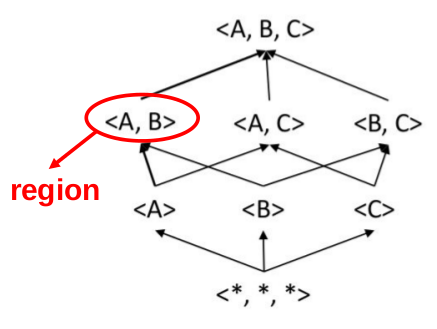
\includegraphics[width=2.1in]{picture/ch_preliminary/abc_lattice} 
\caption{三维数据立方 Lattice}\label{abc_lattice} 
\end{figure} 

在这个lattice中,有维属性组合对应的所有 GroupBy 类型,每个节点表示一种 GroupBy 类型。在lattice中的每个节点称为一个region,也就是一种 GroupBy 类型。箭头连接的两个节点表示它们有父子关系。例如Region(AB)与Region(A)之间有箭头连接,Region(AB)为父,Region(A)为子,表示GroupBy(A)的结果可从GroupBy(AB)的结果计算获得。

一个 region 内有多个 group。group 指的是一个
region中带有具体值的 GroupBy。如表\ref{groupby_a_table}是Region(A)(即GroupBy(A)) 中的group。表中第一列A为属性A的值,第二列M为度量属性聚合计算后的值。在表中,Region(A) 有5个Group,分别是Group(A=0), Group(A=1), Group(A=2), Group(A=4), Group(A=6)。

\begin{table}[!ht]
\begin{center}
\begin{tabular}{|c|c|}
\hline 
A & M \\ 
\hline 
0 & 50 \\ 
\hline 
1 & 100 \\ 
\hline 
2 & 60 \\ 
\hline 
4 & 70 \\ 
\hline 
6 & 90 \\ 
\hline 
\end{tabular} 
\end{center}
\caption{GroupBy(A)}\label{groupby_a_table}
\end{table}


%从lattice中可见,当一个事实表有 D 个维属性时,它对应的数据立方就会有${2}^{D}$个region,也即有 ${2}^{D}$ 种不同类型的 GroupBy。最简单直接(Naive)的数据立方实现方法,是对每个region进行独立计算并把结果存储起来。对于一张事实表,随着他的维属性数量的增加,它相对应的数据立方的计算与存储代价就会呈指数增长。于是,在 OLAP 中,如何从立方计算、立方存储这两个角度高效地实例化数据立方已成为业界内广泛讨论的一个研究课题。


\subsection{度量}

度量,即对GroupBy的多条数据进行聚合计算,例如SUM,AVG,MEDIAN,DISTINCT,TOPK等。

度量函数分为两大类, 分别为代数度量(Algebraic)和整体性度量(Holistic)。

以下使用一个二维的数据集$\left\{ {X}_{ij}|i=1,...I; j=1,...J \right\}$分别说明这两种度量函数的区别。

\begin{itemize}

%\item \textbf{分布度量}
%对于分布度量函数 F(),如果存在一个辅助函数 G() 能令 $F(\text\{ {X}_{i,j} \text\}) = G(\text\{ F(\text\{ {X}_{i,j}|i=1,...,I \text\})|j=1,...J \text\})$,则度量函数 F() 为分布度量函数。常见的分布度量函数有 COUNT(), MIN(), MAX(), SUM()。大部分分布度量函数中 $F=G$,但COUNT() 除外。在COUNT()度量函数中,$G=SUM()$。

\item \textbf{代数度量}

对于代数度量函数 F(),如果存在两个辅助函数 G() 和 H(),其中 G() 的输出结果是固定数量的 M 条记录,并且满足$F(\text\{ {X}_{i,j} \text\}) = H(\text\{ G(\text\{ {X}_{i,j}|i=1,...,I \text\})|j=1,...J \text\})$。常见的代数度量函数有SUM(),COUNT(),AVG(),MaxN(),MinN(),标准差等。例如对于AVG(),函数G()的输出是子集的和以及数量,函数H()则将各个子集的和相加再除以数量的总和。代数度量的关键是,函数G()的输出结果的数据量是固定的。例如对于AVG(),无论数据怎么划分,函数G()的输出都是两个值,一个是和,另一个是数量。

\item \textbf{整体性度量}

对于整体性度量函数 F(),其中间结果,即各个子集的计算结果的数据量大小是不确定的。常见的整体性度量有Median(), Mode(), RANK(), DISTINCT()等。例如使用 DISTINCT()计算一个数列中出现多少不同的数值。若将该数列随意划分,那么每个子数列输出的中间结果仍可能是一个列表,该列表记录了子数列出现哪些数值,即将重复的数值去除。然后再对这些中间结果计算 DISTINCT()。在最坏的情况下,每个子数列输出的中间结果可能就是它本身,因为无重复的数值。

\end{itemize}



%之所以要对度量函数进行分类是因为其会影响数据的划分以及数据立方的计算。论文研究的环境是分布式,因此数据划分是必然的。对于以上三种度量,在分布度量与代数度量下,数据无论如何划分,使用辅助函数都能计算出最终结果,并且中间结果的数据量是确定的。但对于整体性度量,数据无法随意划分,或者数据的随意划分对其计算的意义并不大,因为中间结果数据量的不确定导致中间数据的维护代价可能很大。然而这并不代表数据不能划分。在后面的章节中会提到,对于整体性度量按照一定的方法对数据进行划分,也能令中间结果的数据大小是确定的。为了方便,在之后的阐述中,将分布度量与代数度量都归为代数度量。

%\subsection{MapReduce}

%MapReduce \cite{dean2008mapreduce} 是Google提出的一个分布式计算架构,用于大规模数据集的并行计算。它分为Map和Reduce两大阶段。Map阶段对输入的每一个键值对进行处理,并且输出一个或多个键值对。在Reduce阶段,具有相同key值的键值对会被分派到同一个reduce函数内进行合并计算,并输出最终的计算结果。



\section{国内外概况}

数据立方的计算即是计算事实表中维属性对应的所有组合的GroupBy。最简单的方法是通过扫描原数据逐个 GroupBy 地计算,但是这样的方法效率非常低。而数据立方计算的关键是利用各个 GroupBy 之间的共享关系进行计算。例如一个四维的数据立方,维属性为ABCD,对于Region(A)中各个 group 的计算,可从原数据扫描计算获得,也可从已计算好的Region(AB) 中计算获得,显然从后者计算获得的效率要比前者高得多,因为Region(AB)的数据量一般情况下要比原数据少得多。因此各种数据立方计算方法都是利用 region 之间的一些共享关系解决不同场景不同需求下数据立方的实例化问题。\cite{morfonios2007rolap}


\subsection{单机数据立方计算}

PipeSort\cite{agarwal1996computation} 与 BUC(BottomUpCube)\cite{beyer1999bottom} 是分别由 Agarwal 与 Beyer 于90年代提出的数据立方计算方法,并且仍然是当前较为流行且通用的计算方法。虽然这两种方法在提出时是基于单机实现的,但它们的计算思想对当前分布式数据立方计算有着非常重要的影响。

PipeSort是一种自顶向下的计算数据立方的方法,而BUC是自底向上的。这里的顶与底指的是 lattice 的顶部与底部的 region。PipeSort多用于没有阈值限制的数据立方计算,而BUC则多用于有阈值限制的计算。

对于PipeSort,Pipe指Pipeline,即流水线。它利用数据的有序性以及多个 group 之间具有共同前缀的特性,对数据只扫描一遍并且使用少量的内存即可计算多个 group 的聚合。例如对于 $ABCD\rightarrow ABC\rightarrow AB\rightarrow A$ 这个Pipeline,由于数据已经按照属性ABCD进行排序,因此只对数据进行一次扫描即可计算这条Pipeline 中所有的group。

BUC 算法利用度量函数的单调性,多用于计算有阈值限制的数据立方,如HAVING COUNT(*) > 100 这样的阈值限制。它会根据维属性对基表数据进行多次递归分组并计算聚合结果。在递归的过程中,若发现一些group不满足阈值限制,那么与之相关的 group 就不需要计算了。例如对于COUNT(*) > 100的限制,若计算 Group(A=a0)的COUNT(*)是小于 100 的,那么与 A=a0 相关的 group 就不需要计算了。

根据不同的数据特征以及数据立方的使用场景,\cite{han2001efficient} \cite{harinarayan1996implementing} \cite{xin2003star}  \cite{zhao1997array}  \cite{wang2002condensed} \cite{ross1997fast} 提出了对数据立方计算的改进与优化。\cite{han2001efficient} 对BUC算法进行了改进; \cite{harinarayan1996implementing} 提出为了节省存储空间与计算资源,只计算部分的数据立方; \cite{xin2003star} 是将自顶向下与自底向上的数据立方计算方法相结合;\cite{zhao1997array} 解决基于数组存储的数据进行数据立方的计算;\cite{wang2002condensed} 提出了浓缩数据立方的思想;\cite{ross1997fast} 提出了对lattice进行划分的方法。


\subsection{分布式数据立方计算}

以上的这些方法提出时都是基于单机计算数据立方的。\cite{ng2001iceberg} \cite{dehne2002parallelizing} 提出了在小集群上的并行数据立方计算的方法。但这些方法并没有与MapReduce框架相结合,并且随着数据量的急剧增长,单机和小集群上的计算方法已无法满足数据立方的计算要求。

MapReduce \cite{dean2008mapreduce} 是Google提出的一个分布式计算架构,用于大规模数据集的并行计算。它分为map和reduce两大阶段。map阶段对输入的每一个键值对进行处理,并且输出一个或多个键值对。在reduce阶段,具有相同key值的键值对会被分派到同一个reduce函数内进行合并计算,并输出最终的计算结果。分布式数据立方计算正是可以利用reduce的功能,将同一个group或者同一条Pipeline的数据都放在同一个reduce函数内进行合并计算。

\cite{abello2011building} \cite{wang2010mapreducemerge} \cite{sergey2009applying} \cite{lee2012efficient} 将数据立方的计算与MapReduce相结合,但这些方法都着重解决代数度量函数的计算,并没有考虑整体性度量函数与MapReduce结合时会产生的一系列问题,包括reducer负载不均衡、中间数据过多等问题。由于整体性度量函数的中间数据的数据量是不确定的,很多情况下甚至是无法压缩的,因此使用MapReduce计算整体性度量函数时会出现中间数据过多的问题。同时,由于数据立方中各个group的大小是有差异的,在倾斜数据集中,这些group的大小差异会更为明显。当这些group被分发到各个reducer上进行计算时,由于group大小的差异令各个reducer负载不均衡,从而导致计算效率的下降。

Raghu Ramakrishnan 团队提出的 MapReduce DataCube 方案 \cite{nandi2012data} \cite{nandi2011distributed}(以下简称MR-Cube),是当前 MapReduce 与数据立方的最佳结合。MR-Cube解决了整体性度量函数与MapReduce的结合、数据划分、中间数据过多、合并计算等问题。它通过采样的方式确定数据集中是否有大group,从而对该region内所有的group进行划分,令划分后的每个group都在reducer可处理的数据量范围内,减少MapReduce负载不均衡的情况。同时它还提出了 BatchArea 的概念,将多个 group 放在同一个 reduce 函数内计算,减少中间数据的产生,从而加快数据立方的计算。

虽然 MR-Cube 实现了数据立方与 MapReduce 的高效结合,但其仍存在缺陷,尤其是在一些倾斜的数据集下,该算法的数据划分方法分会产生不必要的划分。并且MR-Cube使用取模的方法划分数据,在一些情况下会导致不均匀的划分。同时它对合并计算只给出了一些建议遵循的规则,并没有给出具体的简单有效的合并方法。此外,MR-Cube 使用了 BUC \cite{beyer1999bottom} 的算法计算 MapReduce 下的数据立方,然而数据立方的实现技术除了 BUC 外,还有 PipeSort,PipeHash \cite{agarwal1996computation} 等。这些方法与 BUC 相比,更能利用 MapReduce 框架的特性。因此可使用其他数据立方计算方法取代 BUC,从而使数据立方计算与MapReduce有更好的整合。

\section{论文主要工作及贡献}

本文探讨当前数据立方计算的研究现状,主要针对Raghu Ramakrishnan 团队提出的 MR-Cube 方案 \cite{nandi2012data} \cite{nandi2011distributed},分析其优缺点,并根据 MR-Cube 的不足以及可改进的地方,主要包括数据划分与合并计算两个方面,提出 TSP-Cube 算法。TSP-Cube 借鉴\cite{tao2013minimal} 中将TeraSort 与 GroupBy 结合的方法进行数据划分,并且根据 MapReduce 特性,采用 PipeSort 计算数据立方,将数据立方的计算与 MapReduce 充分结合。

TSP-Cube 借鉴 Tera Sort 的思想提出更具有通用性的划分方法。TSP-Cube 通过对数据采样与选取分界点的方法划分数据,与MR-Cube中使用取模的方法相比,这种划分方法无论在均匀或是倾斜的数据分布下,都可均匀地划分数据,从而令各个reducer负载均衡。由于 TSP-Cube 是通过数据出现的频率确定要划分的group,因此在保证大group被划分的同时,又可减少甚至避免不必要的数据划分。

TSP-Cube 使用 PipeSort 替代 BUC 方法实现基于 MapReduce 的数据立方,从而更充分地利用MapReduce框架的特性。因为在MapReduce中,reducer的迭代器仅能对数据扫描一次,若要对数据进行多次扫描,则需要将数据载入内存或者再次读写文件,加重了I/O操作。BUC因为需要不断地对数据递归分组,会对数据进行多次扫描,而PipeSort只需对数据进行一次扫描即可计算 Pipeline 上所有的group,因此 PipeSort 比 BUC 更适用于MapReduce。同时,TSP-Cube 针对层次型的数据集以及结合 PipeSort 的特性,提出简单且有效的Pipeline生成方案。

在TSP-Cube章节中,会分别讨论TSP-Cube与代数度量和整体性度量的结合。但由于代数度量与MapReduce已有较好的结合,并且MR-Cube是针对整体性度量提出的算法,因此TSP-Cube也着重解决整体性度量函数计算与MapReduce框架结合的问题。

最后通过实验比较TSP-Cube与多种数据立方计算方法在性能、负载等方面的优势。实验表明,TSP-Cube在计算整体性度量函数时,与其他方法相比,在性能上以及负载均衡上均有明显的优势,且TSP-Cube更具有通用性,适用于均匀以及倾斜的数据分布。实验还包括了多种方法计算代数度量函数的比较,从而根据实验结果总结出两种不同类型的度量函数适用的数据立方计算方法。

%从而为后续的MapReduce 与数据立方计算的优化实现提供研究经验支持。

\section{论文结构安排}
本文内容安排如下,第2章探讨当前数据立方计算的研究现状,分别从分布式与单节点两方面探讨,重点分析MR-Cube的贡献以及不足,为TSP-Cube的提出提供理论依据;第3章提出TSP-Cube算法,分别从使用TeraSort进行数据划分以及使用PipeSort进行合并计算两方面进行详细的理论分析;第4章阐述TSP-Cube与多种算法比较的实验结果与结果分析;第5章总结本文的工作,并提出对未来工作的展望。

